%\documentclass[12pt, a4paper, parskip=half, headings=small, draft=true]{scrartcl} % [10pt, twocolumn] (Schnellübersicht goo.gl/AS72B)
\documentclass[10pt, a4paper]{scrartcl} % Std 11pt % 10 pt!!!
\usepackage[T1]{fontenc} % Umlaute
\usepackage[utf8]{inputenc} % Textcodierung
\usepackage[english]{babel} % Silbentrennung
%\usepackage{marvosym, amsmath, amssymb} % Symbole, Formeln, amssymb > mathdesign
\usepackage{lmodern, microtype} % enhanced CM, mikrotypografische Feinheiten
\usepackage[in]{fullpage} % Ränder [in|cm]
%\usepackage{graphicx, listings} % Grafiken, Quelltext
\usepackage[hidelinks]{hyperref} % Hyperlinks
%\usepackage[dvipsnames]{xcolor} % Farben (goo.gl/sP8iP, S.38)
%\usepackage[charter]{mathdesign} % Schriftart B. Charter
%\usepackage{mathptmx} % Schriftart Times
\usepackage{booktabs}
\usepackage[autolanguage]{numprint}

% ``quotation marks''

\usepackage[firstpage]{draftwatermark} % [final]
\SetWatermarkLightness{0.9}

\usepackage{csquotes} % Recommended addition for biblatex
\usepackage[style=numeric,backend=biber]{biblatex}
\addbibresource{thesis.bib}

\let\origunderscore\_
\renewcommand{\_}{\origunderscore\allowbreak}
\newcommand{\config}[1]{\texttt{config.\allowbreak #1}}

\begin{document}
\begin{titlepage}
\begin{center}
\large{Lehrstuhl für IT-Sicherheitsinfrastrukturen, Informatik 1\\
Friedrich-Alexander-Universität Erlangen-Nürnberg}

\vspace{2cm}
\textbf{\Large{Bachelor Thesis}}

\vspace{1cm}
\textbf{\textsf{\huge{Analysis of BitTorrent Trackers and Peers}}}

\vspace{0.4cm}
\textbf{\textsf{\LARGE{Counting Confirmed Downloads in BitTorrent}}}

\vspace{1cm}
\Large{Stefan Schindler\footnote{Email: stefan@kaloix.de, Student number: 21676746}}

\vspace{1cm}
\Large{Erlangen, \today}

\vspace{6cm}
\large{Examiner: Prof. Dr.-Ing. Felix Freiling\\
Advisor: Philipp Klein, M. Sc. und Michael Gruhn}

\vspace{2cm}
\large{This work is licensed under the\\
Creative Commons Attribution-ShareAlike 4.0 International License.\\
To view a copy of this license, visit\\
\url{http://creativecommons.org/licenses/by-sa/4.0/}.}
\end{center}
\end{titlepage}

\tableofcontents

\listoffigures

\listoftables
\newpage

\section{Introduction}
[Some general information on the context and setting]

\begin{itemize}
  \item BitTorrent by Bram Cohen 2008, a decentral network
  \item BitTorrent traffic statistics
  \item Other file sharing technologies
\end{itemize}

\subsection{Motivation}
[Specific motivation for the problem at hand]

\begin{itemize}
  \item General statistics about illegal usage of BitTorrent
  \item Unique peers vs observed downloads as lower bound
  \item Gather statistics without up- or downloading content
\end{itemize}

\subsection{Task}
[Concrete task to be solved]

\begin{itemize}
  \item Tool: Evaluate one or multiple given torrents
  \item Tool: Count observed downloads per hour
  \item Tool: Determine download speeds of peers
  \item Tool: Group them after geographical territories using IP address geolocation
  \item Drawback: One can only derive lower bounds from observing peers using the standard BitTorrent protocol
  \item Drawback: There is no complete overview about all running torrents, we need to choose a subset
  \item Evaluation: Choose interesting torrents for analysis from different content categories
  \item Evaluation: Run analysis tool for several days or weeks
\end{itemize}

\subsection{Related Work}
[Other relevant academic work and how it differs from this work]

\begin{itemize}
  \item \cite{watters2011much}
  \item \cite{drachen2011distribution}
  \item \dots
\end{itemize}

\subsection{Results}
[What has been achieved in this work?]

\dots

\subsection{Outline}
[How is the thesis structured and why?]

\dots

\subsection{Acknowledgments}
[A big thank you for the support to ...]

\dots

\section{Background}
This chapter explaines technologies and specifications utilized during this research project.

\subsection{BitTorrent Protocol}
Besides several extensions, BitTorrent still works as designed by \textsc{Bram Cohen} in January 10, 2008, in the \emph{BitTorrent Enhancement Proposal} number 3 \cite{bep3}. It establishes a method to distribute a predefined set of files among an arbitrary number of recipients without overwhelming load on a central entity. This is achieved by splitting the file set in pieces and let peers send them to each other. Three main parts are defined to enable the process: The BitTorrent file format containing identifying metadata about the file set, the communication procedure with a tracker server where peers can learn Internet Protocol addresses of other peers, and the peer wire protocol spoken between peers.

\subsubsection{Bencoding}
In order to store common data structures as well as transmit them over TCP, encoding is required to preserve the data's type and semantic. To realize BitTorrent, \textsc{Cohen} came up with \emph{bencoding} to annotate data appropriately. Any integers and length information is encoded in base 10 ASCII format. All types but strings have specific beginning and ending delimiter characters. Basic supported data types are byte strings and integers, saved as \texttt{<length>:<string>} and \texttt{i<integer>e} respectively. Composite types include lists stored as \texttt{l<value1><value2>e} and dictionaries alike \texttt{d<key1><value1><key2><value2>e}. Note that only strings can be used as dictionary keys.

\subsubsection{Metainfo File}
Metadata about a downloadable file set is stored bencoded in a metainfo file, which uses the \texttt{.torrent} file name extension. The purpose is to locate the tracker server and describe all content pieces with cryptographic hashes. Data is arranged in dictionaries of the following structure:

\begin{description}
  \item[announce] Uniform resource locator of the tracker server, usually of the form \nolinkurl{http://<host>:<port>/announce}.
  \item[info] The info dictionary describing the torrent's pieces
  \begin{description}
    \item[name] Optional file or directory name
    \item[piece length] Number of bytes per piece
    \item[pieces] Concatenation of raw SHA-1 hash values for every individual piece
    \item[length] Only present if the torrent is a single file; file size in bytes; not used in this project at all
    \item[files] Only present if the torrent contains multiple files; list of dictionaries, one per file; not used in this project at all
    \begin{description}
      \item[length] File size in bytes
      \item[path] List of subdirectory names and filename representing a path
    \end{description}
  \end{description}
\end{description}

The number of pieces can be derived from the \texttt{pieces} key of the \texttt{info} dictionary by dividing it's length by 20, since a SHA-1 hash is 20 bytes. The torrent identifying \emph{info hash} is calculated as the SHA-1 hash of the bencoded info dictionary.

\subsubsection{Tracker Server}
The biggest problem of BitTorrent is to learn about the contact information of fellow peers. The traditional solution is a tracker server, where peers announce their participation in the torrent swarm and receive a list of other peer's IP addresses and port numbers in one step. Communication with the tracker server is done via the GET request method of the Hypertext Transfer Protocol. The request is sent with the following parameters, whereby keys and values must be quoted using percent-encoding \cite[§~2.1]{percent}.

\begin{description}
  \item[info\_hash] SHA-1 hash of the bencoded info dictionary from the metainfo file
  \item[peer\_id] String of 20 bytes self chosen by each peer; contains client software information by convention
  \item[ip] Optional parameter with the peer's own IP address
  \item[port] Port number this peer is listening on for connections from other peers; recommended ports are 6881 to 6889
  \item[uploaded] Amount of uploaded pieces so far
  \item[downloaded] Amount of downloaded pieces so far
  \item[left] Amount of pieces left to download
  \item[event] Optional key about the circumstances of this request; is \texttt{started}, \texttt{completed} or \texttt{stopped}
  \item[compact] To save bandwidth, a compact list of peers can be requested \cite{bep23}; is \texttt{0} or \texttt{1}
\end{description}

The tracker's response message should contain a bencoded dictionary in the message body. Following keys are defined:

\begin{description}
  \item[failure reason] In case of failure, human-readable error message explaining why the request could not be fulfilled
  \item[interval] Suggested interval in seconds the client should wait between tracker requests
  \item[peers] List of dictionaries, one per peer
  \begin{description}
    \item[peer id] Self-selected ID
    \item[ip] IP address
    \item[port] Port number
  \end{description}

  In case of a compact peer list, this is a single byte string instead of a list of dictionaries. 6 bytes per peer are used containing 4 bytes for the IPv4 address and 2 byte representing the port number.
\end{description}

\subsubsection{UDP Tracker Protocol}
Tracker servers are the only centralized infrastructure required by traditional BitTorrent. Hence it is advisable to reduce bandwidth during tracker requests as much as possible. As BEP 23 demonstrates, using the \emph{UDP tracker protocol} instead of HTTP over TCP can reduce traffic by 50\,\% \cite{bep15}. Since UDP datagrams may arrive out of order, the client sends a randomly chosen transaction ID with every request to identify the matching server response afterwards.

\paragraph{connect}
The first step in the UDP tracker protocol is a connect request. A connection ID is sent in return by the server, which must be included in following requests. As it is possible to spoof an UDP packet's source IP address, the server could be abused for a denial-of-service amplification attack against a third party. The need for a connection ID on other requests, which trigger larger responses, renders this impossible. The connection ID is valid within the next minute.

\paragraph{announce}
This announce request includes the same parameters as the HTTP communication described above. Additional parameters are an unused \texttt{key} value and the \texttt{num\_want} value, allowing to specify the amount of returned peers. The announce response again includes a desired request interval as well as a number of active leechers and seeders. Peer's IPv4 addresses and port numbers are included using six bytes each.

\paragraph{scrape}
Finally a scrape request is defined, giving clients access to the numbers of leechers, seeders and completed downloads as reported by the server. There is no guarantee of validity for these values, since they may be manipulated or chosen by the server freely. An error response package containing a human-readable message may be sent by the server at any time.

\subsubsection{Peer Wire Protocol}
The peer protocol is spoken between peers and allows bidirectional communication with predefined messages. At first an initial handshake is exchanged, containing a protocol string, eight bytes reserved for alternate protocol behavior and extensions, as well as the torrent's info hash and the peer's ID. The connecting client sends it's handshake message first. All following messages begin with an overall length prefix, followed by a type identifier and the payload, if appropriate.

The so called \texttt{bitfield} message may be sent immediately after the handshake to indicate which pieces were already downloaded and verified by the peer. With same intentions \texttt{have} messages are sent to all connected clients, if a peer has successfully downloaded a new piece. These are the only two message types relevant in the scope of this work; for completeness, the meanings of further message types are as follows: \texttt{choke} and \texttt{unchoke} express the willingness and possibility to fulfill requests for pieces. Similarly \texttt{interested} and \texttt{not interested} indicate whether a peer would start downloading if unchoked. A bulk of missing pieces can be requested using a \texttt{request} message with begin and end indices, a single piece can be requested using \texttt{piece}. When requests were sent to multiple clients to increase download speed, a \texttt{cancel} message is used to revoke a pieces request.

\subsection{DHT Protocol}
Despite the complete file payload being transmitted from client to client, still a central server keeping track of all peers is needed. However, the mandatory tracker server contradicts the concept of a decentralized file distribution network and, in addition, has to be maintained financially. The \emph{DHT Protocol} \cite{bep5} solves this issue, as it stores peer contact information in a distributed hash table. Participating peers run a separate DHT \emph{node}, which communicate sending bencoded messages over the User Datagram Protocol. The distributed hash table follows the Kademlia design as described by \textsc{Maymounkov} and \textsc{Mazières} in 2002 \cite{kademlia}.

\paragraph{Nodes}
First, a node generates his own random 20 byte identifier, called node ID. The distance between two node IDs is defined as the bitwise exclusive disjunction interpreted as an unsigned integer. Each node maintains a routing table, which maps node IDs to their corresponding node's IP address and UDP port number. The closer node IDs are to the node's own ID, the more nodes are stored in the routing table. Therefore, nodes only know about a limited number of other nodes, with greater detail close to their own identifier.

\paragraph{Lookup}
The process of extracting peers for a given info hash proceeds iteratively. The same distance metric as used between node IDs is used to identify nodes in the routing table with IDs close to the info hash in question. Due to the routing table's structure, contacted peers can return IDs and addresses of even closer nodes. Eventually, nodes will be able to return actual peer contact information, since peers known to download a torrent are stored in a second table, the hash table. Following the same scheme used on the routing table, peers with info hashes close to the own node ID are stored preferably.

\paragraph{Announcing}
When a peer downloads a torrent, it should announce the info hash and BitTorrent port to multiple other nodes in order to be included in the distributed hash table. Again, the problem of IP address spoofing exists, allowing malicious hosts to register third parties for a torrent. This is why a token system is used. On every successful request for peers, the response includes the SHA-1 hash of both the source IP address and a secret value. The recipient's IP address and the IP address included in the hash are now guaranteed to be equal. When announcing download participation, a node must include this token, allowing the contacted node to verify the announce request's source IP address and updating it's hash table.

\paragraph{Integration}
The presence of DHT support is advertised in the standard BitTorrent handshake of the Peer Wire Protocol using the last bit of the eight reserved bytes. Peers receiving this indicator should send a \texttt{port} message, containing their own UDP node port number. This technique helps populate routing tables, especially on newly installed systems with an empty table.

\subsection{Magnet Link}
The concept of a \emph{magnet link} described in BEP 9 \cite{bep9} is used to create a uniform resource identifier for torrents of minimal size, in comparison to the metainfo file format. It's only mandatory component is the info hash, the SHA-1 value of the info dictionary. The link uses the \texttt{magnet:} URI scheme and stores info hash, a display name and tracker announce URLs in the query string. The emerging problem is the loss of the info dictionary's content. Since a tracker URL is optional, the metadata must be obtained from other peers.

\subsubsection{Extension Protocol}
To expand the functionality of the BitTorrent Protocol, the \emph{Extension Protocol} was defined \cite{bep10}. It introduces the generic \texttt{extended} message to the Peer Wire Protocol, which itself can have various subtypes depending on which extensions are actually used. Extension Protocol support is indicated in the standard Peer Wire Protocol handshake by setting the 20th bit from the right of the eight reserved bytes.

When both peers ascertain support for the Extension Protocol, extended messages containing a second handshake are exchanged. The handshakes contain a dictionary with one or multiple keys: First, a bencoded dictionary \texttt{m} with names of supported extensions together with randomly assigned extension IDs and secondly, additional keys depending on the used extensions. This setup allows for an arbitrary number of extensions with dynamic IDs, without the need for a global registry of extensions. Further extended messages contain the extension ID and payload as defined by the respective extension.

\subsubsection{Extension for Peers to Send Metadata Files}
The \emph{Extension for Peers to Send Metadata Files} \cite{bep9} with identifier \texttt{ut\_metadata} is the first and only extension described here to make use of the Extension Protocol. It places one additional item in the handshake dictionary, namely \texttt{metadata\_size}, containing the size of the bencoded info dictionary in bytes. For transmission, the bencoded info dictionary is divided in pieces of 16 kibibytes. The number of metadata pieces follows from the \texttt{metadata\_size} parameter.

To gather initial contact information of peers to be asked for metadata, the DHT protocol may be used. Then every piece must be requested separately from these peers, using a \texttt{request} message. These are answered by the same number of \texttt{data} or \texttt{reject} messages, depending on whether the opposing client is able to deliver the piece. When all pieces are present, they can be composed and checked against the info hash value.

\subsection{BitTorrent and German Law}
\subsubsection{Illegal Content}
While there are no legal restrictions on using BitTorrent in general, the download of content without permission of the author or right holder is considered an illegitimate reproduction according to the German Copyright Act \cite[art.~15\,(1),~16]{urhg}. The common exception of private copying \cite[art.~53]{urhg} is not applicable here, since the source is ``obviously unlawfully-produced''.

Even more serious is the upload process always involved in BitTorrent. Illegitimate distribution of proprietary content may be sentenced with imprisonment or a fine \cite[art.~106]{urhg}. More common and often abused \cite{abmahnung} is the system of special notifications \cite[art.~97a]{urhg}, sent from right holders to assumed copyright infringers. These warning letters are supposed to settle the controversy extrajudicial in exchange of a fee. Entitlement of right holders to indemnity and expense allowance exists \cite[art.~97]{urhg}.

\subsubsection{Collecting IP addresses}
Privacy is regulated by the Federal Data Protection Act \cite{bdsg} in Germany. It introduces a concept of personal data which includes ``any information [...] of an [...] identifiable individual'' \cite[sec.~3\,(1)]{bdsg}. The collection of personal data is inadmissible without consent of the concerned person \cite[sec.~4]{bdsg}; other exceptions permitted by this Act do not apply. It is disputed whether IP addresses are within the definition of personal data \cite{ip}, so to comply with the law by all means the anonymization of IP addresses is preferable.

\section{Implementation}
The software tool written for this thesis was developed using the version control system \emph{Git} \cite{git} in conjunction with a private online repository provided by \textsc{GitHub}. The source code was published \cite{btda} under the \emph{GNU General Public License} in version 3.

\subsection{Dependencies}
There are a few external dependencies, which are all free and open-source software. The \emph{BencodePy} project by \textsc{Eric Weast} \cite{bencodepy} provides an encoder and decoder for bencoding messages and values. The \emph{Object Relational Mapper} of \emph{SQLAlchemy} \cite{sqlalchemy} is used to store evaluation results in the \emph{SQLite} database format \cite{sqlite}. The \emph{GeoIP2 API} \cite{geoip2-api} is used to perform IP geolocation lookups in the \emph{GeoLite2 City Database} \cite{geolite2-db}. This database is provided by \textsc{MaxMind, Inc.} under the \emph{Creative Commons Attribution-ShareAlike 3.0 Unported License}. In order to run a dedicated DHT node, the tool \emph{pymdht} by \textsc{Raul Jimenez} \cite{pymdht} is used.

\subsection{Functionality}
To count confirmed downloads by peers of one or multiple given torrents over a time period, the \emph{BitTorrent Download Analyzer} was written in Python 3. Torrents and all configuration parameters have to be provided at start, as they cannot be changed later. The program stores results in a SQLite database and runs until manual termination. A configuration file with several variables named \texttt{config.py} is provided. For simplification these variables will be referred to with the prefix ``\texttt{config.}'' in the following, so \config{x} translates to variable \texttt{x} in the configuration file.

The main task is to count confirmed downloads by peers of a given torrent. A download is considered as confirmed, when a peer crosses a threshold of downloaded pieces as defined in \config{torrent\_complete\_threshold}. Thus there must be contact with a peer at least twice -- with the amount of downloaded pieces once below and once equal or above the threshold -- in order to be counted. To determine the download progress of as many peers as possible, two tasks have to be done: First, establish contact to peers from every possible source. Second, receive continuous and reliable information about the download progress of every peer.

For reference, a scrape request is sent to the tracker server every few minutes in order to compare our own counting of peer downloads with numbers as reported by the tracker server.

\paragraph{Import Torrents}
Beforehand, the torrents to be analyzed must be imported. Since both magnet links and torrent files are supported, there are two major ways to do this: All torrent files must be placed in a common directory, specified by \config{input\_path}. They are detected by their \texttt{.torrent} file name extension. Following the specification of BitTorrent files \cite{bep3}, the announce URL, info hash, pieces count and pieces size are extracted.

All magnet links \cite{bep9} to be considered must be placed in a file defined by \config{magnet\_file}, one per line. Since magnet links do not contain the amount and size of the torrent's pieces, but only their info hash, this information must be retrieved from the swarm of other peers. A few peer addresses are gathered with a DHT lookup, then peers are contacted sequentially until the info dictionary could be received using the Extension Protocol \cite{bep10} and the \emph{ut\_metadata} extension \cite{bep9}. The metadata and source of each imported torrent is stored the database for later reference.

\paragraph{Contact Peers}
Sources for peer's IP addresses and port numbers include announce requests to the tracker server as well as lookups in the BitTorrent DHT network. Both are done in dedicated threads and periodically as defined by \config{tracker\_request\_interval} and \config{dht\_request\_interval}. The received peer addresses are filtered for duplicates and placed in a common queue. Each request procedure is recorded in the database with the number of received peers, duplicate peers and duration for further analysis.

Every peer in the queue has a timestamp assigned and must not be contacted prior to this time. When placed in the queue first, the timestamp is set to the current time. Peers in the queue are visited in parallel, whereby the number of threads can be set in \config{peer\_evaluation\_threads}. The queue is sorted ascending, so if timestamps lie in the past the peer which is due the longest time is chosen, if timestamps lie in the future the thread will wait until the attached time is reached. For threads to be able to react to new peers, waiting is capped to \config{evaluator\_reaction}. When the limit is reached, the peer is put back in queue and another one will be chosen.

When a peer with permitted timestamp is picked, a TCP connection is established and the download progress evaluation initiated. Additionally, incoming connections from peers trying to download pieces are used to gather their download status. Therefore a TCP server is listening on the the port defined in \config{bittorrent\_listen\_port}. On successful download progress extraction results are written to the database and IP address port tuples are linked to their database ID in internal memory for later database updates. Failed contacts or peers with unknown info hashes are ignored.

\paragraph{Evaluate Download Progress}
Once a connection is established with a peer, it's download progress must be determined only using peer messages as defined by the BitTorrent Protocol \cite{bep3}. Since there is no dedicated request command for the number of available pieces, we depend on peer messages sent voluntary by the remote peer. Fortunately it is common to advertise available pieces right after the BitTorrent Protocol handshake with \texttt{bitfield} and \texttt{have} messages. These are stored for every peer contact in a separate queue and processed by another thread. Messages are received until a timeout defined by \config{network\_timeout} hits, which is restarted after every message. Additionally there is a limit on the number of messages named \config{receive\_message\_max} to prevent infinite sessions.

Now the only possible approach to acquire the download progress is to compile a combined bitfield from these messages and count the present pieces. The number of total torrent pieces from in the info dictionary helps validating the results.

\paragraph{Peer Database}
With reference to the peer's database identifier, the IP address and port number are saved in the internal memory in order to update an already stored peer entry in the database at later contact. Time and pieces count only of the first and the last peer contact are saved in the database, since this is enough to assess the transition of the confirmed download's threshold. Additionally the download speed is calculated between each two consecutive contacts, whereby only an overall maximum is kept.

Other information about peers stored in the database include an anonymized IP address, the BitTorrent Protocol peer ID, top and second level domain of the hostname, IP geolocation with city, country and continent as determined by the \emph{GeoIP2 API} \cite{geoip2-api}, number of contacts and the original source of the peer's IP address. Afterwards the peer's queue timestamp is updated with the current time plus \config{peer\_revisit\_delay} and it is returned to the queue if \config{torrent\_complete\_threshold} is not reached.

\paragraph{Secondary Statistics}
In order to enable and proof validity of test results some statistics are logged at a certain interval defined in \config{statistic\_interval}. These are the length of the peer queue, length of the queue of visited peers, average workload of peer contact threads, mean time for receiving all messages before timeout. Cumulative values are unique incoming peers, successful initiated contacts, failed initiated contacts at first try, failed initiated contacts at later try and successful evaluated incoming peers.

\dots

\noindent\hrulefill

Explain implementation of the features:

\begin{itemize}
\item Import torrents from \texttt{.torrent} files (BEP 3)
\item Import torrents form magnet links by fetching metadata via the \emph{ut\_metadata} extension (BEP 9) using the Extension Protocol (BEP 10)
\item Continuously get IPv4 peers from the tracker using HTTP (BEP 3) and UDP announce requests (BEP 15)
\item Communicate with peers using a subset of the Peer Wire Protocol (BEP 3)
\item Continuously get IPv4 peers by integrating a running DHT node (BEP 5) from the \emph{pymdht} project using local telnet
\item Actively contact collected peers and calculate minimum number of downloaded pieces by receiving all \emph{have} and \emph{bitfield} messages until a timeout
\item Passively listen for incoming peer connections and calculate minimum number of downloaded pieces analog
\item Save number of downloaded pieces from first and last visit and maximum download speed per peer in a SQLite database
\item Save city, country and continent via IP address geolocation
\item Save ISP by hostname and anonymized IP address
\item Analyze multiple torrents at once
\item Synchronized analysis shutdown process
\item Produce extensive log output
\item Save duplicate and timing statistics about peers received via DHT and tracker
\item Save statistics about failed and succeeded peer connections
\item Save workload statistics of active peer evaluation threads
\end{itemize}

\subsection{Architecture}
It is structured in the main script, an application module, five helper modules and an utility module, which will be described in detail.

They have the following roles:

\begin{description}
  \item[\texttt{main.py}] This is the main script to be invoked when performing the analysis.
  \item[\texttt{analyzer.py}]
  \item[\texttt{torrent.py}]
  \item[\texttt{tracker.py}]
  \item[\texttt{dht.py}]
  \item[\texttt{protocol.py}]
  \item[\texttt{storage.py}]
  \item[\texttt{util.py}]
  \item[\texttt{config.py}]
\end{description}

\subsection{Justification of Configuration Values}
\paragraph{\config{network\_timeout}}
The timeout for network operations is six seconds. It is used when asking the BitTorrent tracker or DHT node for peers and when asking other peers for metadata. These cases are uncritical as a failure is visible in the log files and did not happen during this research. The important spot of application is during the peer evaluation process. While all messages are received from a peer, the timeout resets after every message. Message collection is considered to be complete after the timeout finished without receiving a message.

\begin{figure}
\centering
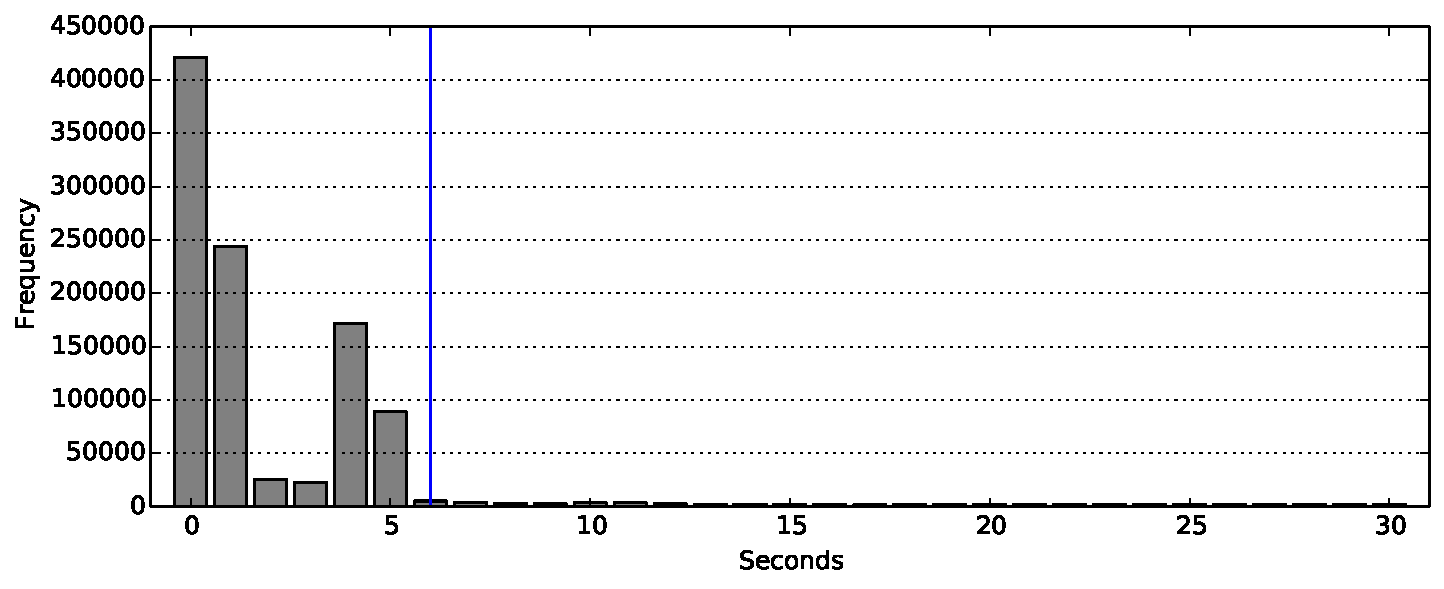
\includegraphics[width=\textwidth]{2015-08-14_17-46-44_faui1-246_timeout}
\caption{Duration to receive one peer message}
\label{timeout-calibration}
\end{figure}

To assess a minimum timeout, an analysis with special configuration parameters was performed\footnote{Files: \texttt{2015-08-14\_17-46-44\_faui1-246.sqlite}, \texttt{2015-08-14\_17-46-44\_faui1-246\_timeout.txt}}. Here the maximum time used for receiving one message was recorded for every peer contact. These durations were rounded and the number of occurrences plotted in figure \ref{timeout-calibration}. For this task \config{network\_timeout} was set to 30 seconds to achieve most unbiased results. During this test at \numprint{977301} out of \numprint{1040817} peer contacts the maximum duration for receiving one message was below six seconds, which equals \numprint[\%]{93.9}.

\paragraph{\config{torrent\_complete\_threshold}}
\dots

\paragraph{\config{peer\_evaluation\_threads}}
\dots

\subsection{Restrictions}

Restrictions and why this does not invalidate the results (hopefully, TBD):

\begin{itemize}
  \item No support for IPv6 on HTTP, UDP or DHT requests
  \item No support for the Micro Transport Protocol ($\mu$TP)
  \item No support for Peer exchange (PeX)
  \item No support for the Tracker exchange extension (BEP 28)
  \item No support for the BitTorrent Local Tracker Discovery Protocol (BEP 22)
  \item No BitTrorrent Protocol support for getting download progress info
\end{itemize}

\subsection{Usage}
pymdht: It must me started seperately and is controlled automatically using a localhost Telnet connection. It could not be integrated directly, since it is written in Python version 2. The desired UDP node port and the Telnet control port must be given as arguments and should reflect the values written in the \emph{BitTorrent Download Analyzer's} configuration file. The typical command used here is \texttt{run\_pymdht\_node.py -{}-port=17000 -{}-telnet-port=17001}. It is sensible to check whether \emph{pymdht} has crashed before and after each analysis run to ensure complete results.

The main script, named \texttt{btda.py} can be controlled by using the following command line options.

\begin{description}
  \item[\texttt{-{}-active <threads>}] Actively contact and evaluate peers using the specified number of threads.
  \item[\texttt{-{}-passive}] Listen on the port specified in the configuration file for incoming connections and evaluate these peers.
  \item[\texttt{-{}-dht}] Integrate and control an already running \emph{pymdht} \cite{pymdht} DHT node using Telnet. The UDP port on which the node is running and the localhost Telnet port where \emph{pymdht} can be controlled are given via \config{dht\_node\_port} and \config{dht\_control\_port} respectively.
  \item[\texttt{-{}-debug}] Write log messages to the console instead of a file and include debug messages.
  \item[\texttt{-{}-help}] Show a help message and exit.
\end{description}

\section{Evaluation}
\subsection{Choosing Torrents}
\begin{table}
\centering
\begin{tabular}{rllr}
\toprule
Rank & Site name & Domain name & Alexa Rank \\
\midrule
1 & Kickass Torrents & \texttt{kat.cr} & 116 \\
2 & ExtraTorrent.cc & \texttt{extratorrent.cc} & 335 \\
3 & Nyaa Torrents & \texttt{www.nyaa.se} & 399 \\
4 & Torrentz Search Engine & \texttt{torrentz.eu} & 464 \\
5 & The Pirate Bay & \texttt{thepiratebay.se} & 507 \\
6 & YTS & \texttt{yts.to} & 669 \\
7 & Rarbg & \texttt{rarbg.to} & 1,150 \\
8 & 1337x & \texttt{1337x.to} & 1,661 \\
9 & EZTV & \texttt{eztv.ch} & 1,831 \\
10 & torrentHound.com & \texttt{www.torrenthound.com} & 2,188 \\
11 & IPTorrents & \texttt{iptorrents.com} & 3,256 \\
12 & isoHunt & \texttt{isohunt.to} & 3,816 \\
13 & Bitsnoop P2P Search & \texttt{bitsnoop.com} & 4,293 \\
14 & Torrent Downloads & \texttt{www.torrentdownloads.me} & 4,315 \\
15 & LimeTorrents.cc & \texttt{www.limetorrents.cc} & 4,552 \\
16 & TamilRockers.net & \texttt{tamilrockers.com} & 4,586 \\
17 & Monova Torrent Search & \texttt{www.monova.org} & 4,843 \\
18 & Torrent Reactor & \texttt{torrentreactor.com} & 5,362 \\
19 & YourBittorrent & \texttt{yourbittorrent.com} & 5,952 \\
20 & TorrentProject & \texttt{torrentproject.se} & 6,670 \\
21 & TorrentFunk & \texttt{www.torrentfunk.com} & 7,682 \\
22 & demonoid.pw & \texttt{www.demonoid.pw} & 7,947 \\
23 & TorrentLeech.org & \texttt{torrentleech.org} & 9,749 \\
\bottomrule
\end{tabular}
\caption{Popularity of torrent directory sites according to Alexa's global traffic ranking}
\label{torrentsites}
\end{table}

To determine most popular torrent directory sites, global traffic rankings by \textsc{Alexa Internet, Inc.} \cite{alexa} were consulted. The websites looked up at Alexa were collected through manual investigation using web search engines, relevant news sites and cross references between sites, because there is no complete list of torrent sites. Table~\ref{torrentsites} shows sites found having an Alexa rank below 10,000 as of July 16, 2015.

\begin{table}
\centering
\begin{tabular}{rllrrr}
\toprule
ID & Site name & Torrent name & Size & Leechers & Seeders \\
\midrule
1 & Kickass Torrents & torrent\_name & 3.0\,GB & 42 & 23 \\
\bottomrule
\end{tabular}
\caption{Most popular torrents of the most popular torrent sites}
\label{torrents}
\end{table}

From the first three sites, the respective five most popular torrents were chosen for analysis. All \textbf{15 torrents} are listed in table \ref{torrents}, with leecher and seeder numbers accurate as of August 42*, 2015.

\subsection{Counting Downloads}
\paragraph{Hardware}
Data collection with the BitTorrent Download Analyzer tool was performed on a virtual machine running Ubuntu 14.04 LTS with 1.0\,GB of RAM, a 3.4\,GHz processor and an own IPv4 address without NAT. The 15 chosen torrents were analyzed at once concurrently using \textbf{512 threads}

\begin{table}
\centering
\begin{tabular}{lrrr}
\toprule
Source & Unique peers & Received peers & Ratio \\
\midrule
Tracker server & 1 & 2 & 3\,\% \\
DHT network & 1 & 2 & 3\,\% \\
Incoming connection & 1 & 2 & 3\,\% \\
\bottomrule
\end{tabular}
\caption{Received peer addresses per source}
\label{unique-peers}
\end{table}

\paragraph{Requests}
The analysis was performed from 11:11 am, August 15 to 11:11 am, August 17, 2015. A time period of 48 hours was chosen in order to detect patters during the day-night cycle. Peers from all sources, namely from the tracker server, the DHT network and incoming connections, were considered. The number of unique peers in regards to their source is shown in table \ref{unique-peers}. The ratio between new and duplicate received peer address information settles after about \textbf{6 hours} at \textbf{76*\,\%}. A history of all peer requests is shown in figure \ref{request-history}.

Request statistics (new/duplicate peers, source of peers, saturation)

The timeline of confirmed downloads and downloads reported by the tracker server in scrape requests is shown in one hour steps in figure \ref{downloads}.

Map: Distribution of downloads (TODO)

Map: Distribution of download speeds (TODO)

\subsection{Further Results}
Diagram: Timeline of new vs. duplicate received peers in 1 hour steps (TODO)

Table: Examine hostnames by ISP or seedbox provicers (TODO)

\section{Conclusion and Future Work}
\dots

\appendix
\section{Evaluation Details}
\subsection{Development of received peer addresses per source}
\label{request-history}
\includegraphics[width=\textwidth, page=1]{2015-07-18_21-57-15_faui1-246_source}\\
\includegraphics[width=\textwidth, page=2]{2015-07-18_21-57-15_faui1-246_source}\\
\includegraphics[width=\textwidth, page=3]{2015-07-18_21-57-15_faui1-246_source}\\
\includegraphics[width=\textwidth, page=4]{2015-07-18_21-57-15_faui1-246_source}\\
\includegraphics[width=\textwidth, page=5]{2015-07-18_21-57-15_faui1-246_source}\\
\includegraphics[width=\textwidth, page=6]{2015-07-18_21-57-15_faui1-246_source}\\
\includegraphics[width=\textwidth, page=7]{2015-07-18_21-57-15_faui1-246_source}\\
\includegraphics[width=\textwidth, page=8]{2015-07-18_21-57-15_faui1-246_source}

\subsection{Confirmed and server reported download numbers}
\label{downloads}
\includegraphics[width=\textwidth, page=1]{2015-07-18_21-57-15_faui1-246_download}\\
\includegraphics[width=\textwidth, page=2]{2015-07-18_21-57-15_faui1-246_download}\\
\includegraphics[width=\textwidth, page=3]{2015-07-18_21-57-15_faui1-246_download}\\
\includegraphics[width=\textwidth, page=4]{2015-07-18_21-57-15_faui1-246_download}\\
\includegraphics[width=\textwidth, page=5]{2015-07-18_21-57-15_faui1-246_download}\\
\includegraphics[width=\textwidth, page=6]{2015-07-18_21-57-15_faui1-246_download}\\
\includegraphics[width=\textwidth, page=7]{2015-07-18_21-57-15_faui1-246_download}\\
\includegraphics[width=\textwidth, page=8]{2015-07-18_21-57-15_faui1-246_download}
\newpage

\printbibliography[heading=bibintoc]
\end{document}
